%%
%% This is file `sample-sigplan.tex',
%% generated with the docstrip utility.
%%
%% The original source files were:
%%
%% samples.dtx  (with options: `sigplan')
%% 
%% IMPORTANT NOTICE:
%% 
%% For the copyright see the source file.
%% 
%% Any modified versions of this file must be renamed
%% with new filenames distinct from sample-sigplan.tex.
%% 
%% For distribution of the original source see the terms
%% for copying and modification in the file samples.dtx.
%% 
%% This generated file may be distributed as long as the
%% original source files, as listed above, are part of the
%% same distribution. (The sources need not necessarily be
%% in the same archive or directory.)
%%
%%
%% Commands for TeXCount
%TC:macro \cite [option:text,text]
%TC:macro \citep [option:text,text]
%TC:macro \citet [option:text,text]
%TC:envir table 0 1
%TC:envir table* 0 1
%TC:envir tabular [ignore] word
%TC:envir displaymath 0 word
%TC:envir math 0 word
%TC:envir comment 0 0
%%
%%
%% The first command in your LaTeX source must be the \documentclass command.
\documentclass[sigplan,anonymous, review]{acmart}

%%
%% \BibTeX command to typeset BibTeX logo in the docs
\AtBeginDocument{%
  \providecommand\BibTeX{{%
    Bib\TeX}}}

%% Rights management information.  This information is sent to you
%% when you complete the rights form.  These commands have SAMPLE
%% values in them; it is your responsibility as an author to replace
%% the commands and values with those provided to you when you
%% complete the rights form.
\setcopyright{acmcopyright}
\copyrightyear{2022}
\acmYear{2022}
\acmDOI{}

%% These commands are for a PROCEEDINGS abstract or paper.
\acmConference[GPCE '22]{21st International Conference on Generative Programming}{December 05--07,
  2022}{Auckland, NZ}
\acmPrice{}
\acmISBN{}


%%
%% Submission ID.
%% Use this when submitting an article to a sponsored event. You'll
%% receive a unique submission ID from the organizers
%% of the event, and this ID should be used as the parameter to this command.
%%\acmSubmissionID{123-A56-BU3}

%%
%% For managing citations, it is recommended to use bibliography
%% files in BibTeX format.
%%
%% You can then either use BibTeX with the ACM-Reference-Format style,
%% or BibLaTeX with the acmnumeric or acmauthoryear sytles, that include
%% support for advanced citation of software artefact from the
%% biblatex-software package, also separately available on CTAN.
%%
%% Look at the sample-*-biblatex.tex files for templates showcasing
%% the biblatex styles.
%%

%%
%% The majority of ACM publications use numbered citations and
%% references.  The command \citestyle{authoryear} switches to the
%% "author year" style.
%%
%% If you are preparing content for an event
%% sponsored by ACM SIGGRAPH, you must use the "author year" style of
%% citations and references.
%% Uncommenting
%% the next command will enable that style.
%%\citestyle{acmauthoryear}

\usepackage{booktabs, multirow} % for borders and merged ranges
\usepackage{soul}% for underlines
\usepackage{comment}
\usepackage{wrapfig}
\usepackage{capt-of}
%A set of custom commands that are used for my personal latex style
%Created: Feb 2020
%Updated: July 2020
\usepackage{listings}

\newcommand{\defn}[1]{\textbf{#1}} %definitions are bold
\newcommand{\jnote}[1]{\textcolor{blue}{Justin: #1\\}} %a note from Justin
\newcommand{\rnote}[1]{\textcolor{orange}{Ron: #1\\}} %a note from Ron
\newcommand{\pnote}[1]{\textcolor{purple}{Peyton: #1\\}} %a note from Peyton
\newcommand{\todo}[1]{\textcolor{red}{TODO: #1\\}} %a todo note

\definecolor{tangerine}{RGB}{245,166,35} %comments, primary color
\definecolor{blueSeaFoam}{RGB}{80,227,194}
\definecolor{liteGreen}{RGB}{184,233,134 }
\definecolor{royalBlue}{RGB}{74,144,226} %keywords
\definecolor{amaranth}{rgb}{0.9, 0.17, 0.31} %special keywords
\definecolor{lavender}{rgb}{0.71, 0.49, 0.86}

\lstdefinestyle{mystyle}{
    backgroundcolor=\color{white},   
    commentstyle=\color{tangerine},
    keywordstyle=\color{royalBlue},
    identifierstyle=\color{black},
    numberstyle=\tiny\color{gray},
    basicstyle=\ttfamily\footnotesize,
    breakatwhitespace=false,         
    breaklines=true,                 
    captionpos=b,                    
    keepspaces=true,                 
    numbers=left,                    
    numbersep=5pt,                  
    showspaces=false,                
    showstringspaces=false,
    showtabs=false,                  
    tabsize=2,
    frame=lines,
    %just for Chisel
    emph={Module, IO, Input, Output, UInt, Bool, Wire, Vec, before, after, extend, in, register, insert, apply, Pointcutter, AfterToken},
    emphstyle=\color{amaranth}
}

\lstset{style=mystyle}


%% Algorithms
\usepackage{algorithm}
\usepackage{algorithmic}
% \usepackage{algorithm2e}
% \RestyleAlgo{ruled}


%%
%% end of the preamble, start of the body of the document source.
\begin{document}

%%
%% The "title" command has an optional parameter,
%% allowing the author to define a "short title" to be used in page headers.
\title{Feature-Oriented Construction of Finite State Machines}

%%
%% The "author" command and its associated commands are used to define
%% the authors and their affiliations.
%% Of note is the shared affiliation of the first two authors, and the
%% "authornote" and "authornotemark" commands
%% used to denote shared contribution to the research.
\author{Justin Deters}
\email{j.deters@wustl.edu}

\author{Peyton Gozon}
\email{peyton.gozon@wustl.edu}

\author{Max Camp-Oberhauser}
\email{c.max@wustl.edu}

\author{Ron Cytron}
\email{cytron@wustl.edu}

\affiliation{%
  \institution{Washington University in St. Louis}
  \city{St. Louis}
  \state{Missouri}
  \country{USA}
}

%%
%% By default, the full list of authors will be used in the page
%% headers. Often, this list is too long, and will overlap
%% other information printed in the page headers. This command allows
%% the author to define a more concise list
%% of authors' names for this purpose.
\renewcommand{\shortauthors}{Deters et al.}

%%
%% The abstract is a short summary of the work to be presented in the
%% article.
\begin{abstract}
We investigate the generation of complex, featureful finite-state machines from relatively simpler ones using two constructs.  The first, inspired by aspect-oriented programming, applies incremental changes to the states and edges of a finite-state machine to alter and customize its behavior in response to features of interest.   This allows efficient specification and generation of numerous designs, each containing only those features of interest for a particular application.

The second construct couples the behavior of multiple finite machines into a single machine that processes its inputs simultaneously.  While this is formally the concatenation of regular languages, we present a \emph{cross-product} algorithm that allows the resulting design to process its wider inputs in lock-step.  This is necessary for the proper timing of actions taken by the resulting machine. 

Each construct is illustrated and results are presented using a simple example:  a vending machine and the game of Nim, respectively.  We then apply the constructs in concert to generate a coherent, $n$-way multiprocessor cache from a much simpler specification.

We show that our approach can generate designs that are exponentially large in the size of their specifications.  In addition to that significant design leverage, the resulting finite-state machines enjoy all the closure properties and proof opportunities for regular languages.
\end{abstract}

%%
%% The code below is generated by the tool at http://dl.acm.org/ccs.cfm.
%% Please copy and paste the code instead of the example below.
%%
\begin{CCSXML}
<ccs2012>
<concept>
<concept_id>10011007.10011006.10011041.10011047</concept_id>
<concept_desc>Software and its engineering~Source code generation</concept_desc>
<concept_significance>500</concept_significance>
</concept>
<concept>
<concept_id>10010583.10010682.10010689</concept_id>
<concept_desc>Hardware~Hardware description languages and compilation</concept_desc>
<concept_significance>500</concept_significance>
</concept>
</ccs2012>
\end{CCSXML}

\ccsdesc[500]{Software and its engineering~Source code generation}
\ccsdesc[500]{Hardware~Hardware description languages and compilation}

%%
%% Keywords. The author(s) should pick words that accurately describe
%% the work being presented. Separate the keywords with commas.
\keywords{feature-oriented programming, finite state machines, generative programming, hardware generation}
%% A "teaser" image appears between the author and affiliation
%% information and the body of the document, and typically spans the
%% page.

%%
%% This command processes the author and affiliation and title
%% information and builds the first part of the formatted document.
\maketitle

\section{Introduction}

The advent of hardware-generation languages like Chisel~\cite{chisel:article} has promoted the adoption of techniques and abstractions by hardware designers that were previously available only to software systems and their designers. As HTML describes the components, structure, and connections of a web page, so do hardware-characterization languages such as VHDL~\cite{vhdl} and Verilog~\cite{verilog} describe the components and interconnections of hardware circuit elements. While those languages provide some abstractions (such as arithmetic operations and restrictive macros), the paradigms and practices used widely in successful software engineering efforts are largely unavailable.

By contrast, hardware-generation languages allow a designer to write a program whose \emph{execution} generates the hardware design. The program can be authored using para\-digms that promote efficiency, reuse, rigorous testing, and clarity of expression. Our work builds on the hardware-generation language Chisel~\cite{chisel:book}, which is in turn built on Scala~\cite{scala-overview-tech-report}. Chisel is a Scala-embedded domain specific language with libraries that generate Verilog when a Chisel program is executed.

% A recent example showing the advantages of hardware generation over characterization concerns an adder~\cite{Deters:adder}. Using VHDL, a hardware designer can request that an adder circuit be optimized for either for delay (carry lookahead) or for area (carry propagate). Using hardware generation, an adder can be specified that combines \emph{both} forms of carry computation, to meet a timing or area constraint, while otherwise optimizing for the other resource.

Chisel has proven itself robust in pedagogy and industry, serving as the basis for courses in digital logic~\cite{vlsicourse} and serving as a platform for describing full-featured RISC-V systems~\cite{chisel:riscv}.  
%Our long-term goal is to develop a feature-oriented characterization of RISC-V~\cite{riscv}.  Here we focus on a specific, more modest construct used in hardware designs.

In this paper, we consider a feature-oriented programing (FOP) approach to generating hardware, specifically \emph{finite-state machines} (FSMs).   Our contributions are as follows:
\begin{itemize}
    \item In Section~\ref{sec:vend}, we describe an approach to formulating features in FSMs based on aspect-oriented programming (AOP).  We apply this idea to a featureful vending machine in Section~\ref{sec:ccut} and present results on the automatically generated FSMs with specific featuere sets in Section~\ref{sec:vendresults}.
    \item In Section~\ref{sec:nim} we introduce a generative approach to composing larger FSMs from smaller, behavior-specific machines, illustrated using the game of Nim.  The algorithm to achieve this \emph{cross-product} composition is presented in Section~\ref{sec:cpalg}, and results from its application to variations of Nim are shown in Section~\ref{sec:nimresults}.
    \item We combine both of the above ideas in Section~\ref{sec:cache} to the generation of an SIMD cache, similar to one currently in use by~AMD.  The parallelism of the cache is generated via the cross-product technique and a coherence scheme is imposed as a feature using the AOP technique.
    \item Theoretically, Sections~\ref{sec:vend} and~\ref{sec:nim} show that a specification of size $O(n)$ can (in the limit) generate variations or structures of size~$O(2^{n})$.  Our results in Section~\ref{sec:results} confirm empirically that our approach offers significant leverage toward generating large, complex FSMs from relatively smaller and simpler ones. 
    \item The FSMs generated by our work are
    \begin{itemize}
        \item correct by construction if the constituent machines and aspectual advice are correct, and
        \item subject to analyses of regular languages, about which much is decidable. 
    \end{itemize}
    \item The code we have developed for this work integrates with Chisel and is available via \texttt{github}~\cite{anon}.
\end{itemize}


\section{Prior work and motivation}\label{sec:prior}

We review here the concepts and prior work upon which our work is based.
\subsection{Aspect-oriented programming}

Our work builds on a programming paradigm available in the software community that efficiently supports the expression and application of \emph{cross-cutting} concerns in a software system.  Aspect-Oriented Programming~(AOP)~\cite{gregor:97} and its realization in systems such as AspectJ~\cite{aspectj} allow developers to express ideas in a software system that affect multiple components of that system in support of a common idea or feature. A commonly cited example is the implementation of a logging feature, so that every method when called and prior to returning logs those events to some output stream. Absent an AOP approach, a developer is faced with the following difficulties:
\begin{itemize}
    \item Implementation of the feature would require modifying every method at its entry and every possible exit so that it emitted the proper log messages.  This is both tedious and error-prone, especially if methods can exit due to unforeseen actions such as exceptions.
    \item Removing the feature, should it no longer be needed, is also tedious and error-prone.
    \item Placing the feature under some kind of conditional execution offers some relief, but
    \begin{itemize}
        \item The conditions themselves incur execution time and the logging code occupies code space.
        \item Subsequent modifications to the system must be mindful to include properly the logging actions.
    \end{itemize}
\end{itemize}
%Macro processors can achieve the proper effect, namely including the code only when it is desired.  However, it is still incumbent on developers to remember to call the macros at the proper points in a program.
AOP is a great solution to this and similar problems, because a developer can specify that at \emph{every} method entry and exit (other than the method that does the logging), a segment of code should be inserted to accomplish the appropriate logging.  If the logging is no longer desired, the associated aspect is simply omitted when building the system.  In this way, both originally and upon modification, all methods' entries and exits are properly logged.

Aspects have been applied to finite-state machines for sequence diagrams in a modeling (UML) setting~\cite{aspectsUML}.  Our use of aspects extends that work by taking advantage of types in Scala to formulate advice and guide FSM modifications. 

\subsection{Benefits of feature-oriented programming}\label{sec:benefop}

Our work concerns the generation of FSMs that incorporate desirable subsets of features.  We show that FSMs can be specified much more efficiently using this approach.  Moreover, the FSMs ultimately generated by the Chisel toolchain contain only those features of interest, requiring fewer resources than would a full-featured, monolithic specification that disables undesirable features.

This approach has also been attractive for managing product lines in which features evolve over time, affecting not only the base system but also other features~\cite{10.1145/2897695.2897701}. 

An example of the benefits obtainable from an FOP approach to a featureful system concerns the CORBA~\cite{CORBA:00} Event Channel~\cite{CORBAService:02a}. The standard implementation is \emph{monolithic}, offering all possible features in all allowable combinations.  A decomposition of the Event Channel in terms of its features has demonstrated that useful subsets of those features use significantly fewer resources when formulated generatively~\cite{Pratap:04}.   

We find that the FSMs we generate enjoy the same benefits as the software systems we describe above:
\begin{itemize}
    \item Smaller footprint (less logic) is obtained by including only those features of interest.
    \item The clock rate of the resulting systems is determined only by active features:  logic related to inactive features is completely absent from the resulting designs.
\end{itemize}

  
\subsection{Decidability}\label{sec:decide}

The theory of regular languages and finite-state machines allows that questions related to properties of the behavior of such machines have definite and algorithmically obtained answers~\cite{sipser}. For example, consider a feature that is intended to \emph{extend} the behavior of a design, so that all previous inputs are allowed, but the feature introduces some other allowable inputs. For example, consider an FSM that scans characters to parse them as decimal numerals.  An extension might allow for hexadecimal numerals, if the input begins with ``0x''.  We would like to prove that the extended language is indeed a proper superset of the original language, which is possible for finite-state machines.  As another example, \emph{timed automata}~\cite{10.1145/2518102} could reason about real-time properties of finite-state machines generated by our approach.

\section{Generative FSM specifications}

We next illustrate our two mechanisms for generating designs.  The first uses aspect-oriented advice to incorporate features selectively into an FSM.  The second builds an FSM from the synchronous simulation of smaller FSMs.

\subsection{Feature introduction via AOP}\label{sec:vend}

As an example of a featureful design, we consider an FSM design for a vending machine.   A state in our design carries the necessary \emph{traits} to represent its role in the machine's operation:  the funds inserted and the potential products dispensed.  Our generative approach described below offers the following advantages over a monolithic design:
\begin{itemize}
    \item The simplest design becomes correct by construction, with states generated automatically based on currency values.  Introduction of a new value of coinage automatically creates the necessary additional states.
    \item Features of interest are easily applied based on states' traits.
\end{itemize}
For this example and the results we present, the features of interest are as follows:
\begin{description}
    \item[Add Currency] introduces a value of coinage.
    \item[Dispense Product] introduces the price of a vendible item.
    \item[Print Funds] display the total funds after each state change.
    \item[Insufficient Funds] advises the user to insert more funds to buy a particular item.
    \item[Change Return] causes the machine to return inserted funds.
    \item[Peanut Warning] requests confirmation of purchase for items that contain peanuts.
    \item[Buy More] allows the user to continue purchasing items if funds remain in the machine.
\end{description}
The dependencies of these features are shown in Figure~\ref{fig:vmDependencies}, but this graph is not needed for construction:  the advice for a given feature is applicable only when its associated \emph{joinpoints} exist in the FSM.  As is typical with aspect-oriented approaches, all advice is presented to the weaver (our runtime library for Chisel), and the aspects are continually applied until no changes occur.

For example, the advice for \textbf{Add Currency} of coinage $k$ specifies that for any state representing that $n$ cents have been inserted, a state representing $n+k$ cents must exist, with a transition from state~$n$ to state~$n+k$ based on the insertion of coinage $k$.   This advice fails to terminate if not capped by some upper bound on funds, which could be related to the most expensive product sold. For example, Figure~\ref{fig:vend1} shows a machine that
\begin{itemize}
    \item Accepts only 5 cent coinage
    \item Accepts up to 15 cents
    \item Vends peanuts that cost 10 cents
\end{itemize}
The FSM is automatically generated by the advice for \textbf{Add Currency} and \textbf{Dispense Product}.  Continuing with this example, consider the \textbf{Buy More} feature, intended to incentivize consumers to spend more money.  This feature causes the machine to retain remaining funds after a purchase to encourage subsequent purchases.  Without this feature, the machine in Figure~\ref{fig:vend1} would return 5~cents if 15~cents are used to purchase peanuts costing 10~cents.  With the feature, the 5~cents of remaining value would be held by the machine for subsequent purchases.  The advice for this feature modifies \emph{every} purchase to move to a state representing currently held funds.  In Section~\ref{sec:ccut} we discuss application of other features to this FSM.

A monolithic approach requires designers to specify all states and transitions for each feature subset, which is tedious and error-prone. With our approach, all states and transitions are obtained generatively and are correct by construction, if the advice for their creation is correct.

In terms of leverage, consider an FSM for which there are $n$ orthogonal and independent features.  A valid system could thus be written or generated with or without each of those $n$ features.  This leads to $2^{n}$ feature-specific implementations.  While it is unlikely that each of those implementations would find an application, the ability to generate \emph{any} of them with the push of a button offers significant leverage.

\begin{figure*}
    \centering
    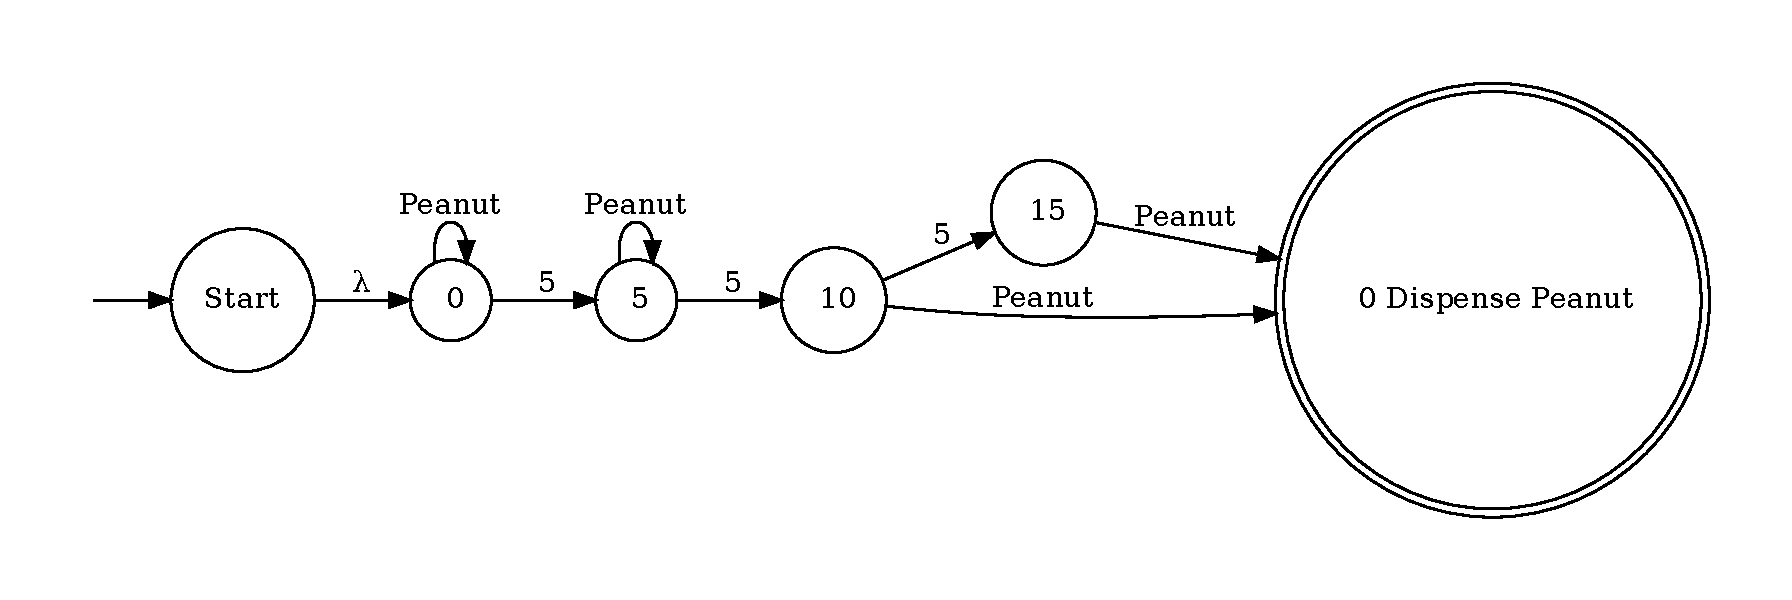
\includegraphics[width=0.7\textwidth]{figures/vend1.pdf}
    \caption{FSM for a vending machine that accepts 5 cent coins and dispenses peanuts that cost 10 cents.}
    \label{fig:vend1}
\end{figure*}

\begin{figure}
    \centering
    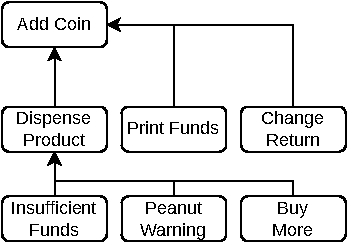
\includegraphics[width=0.55\linewidth]{figures/VendingMachine.pdf}
    \caption{Dependencies between vending machine features.}
    \label{fig:vmDependencies}
\end{figure}

\subsection{Generating FSMs via cross-product composition}\label{sec:nim}

Nim~\cite{enwiki:1102668015} is a broad class of impartial mathematical strategy games, which traditionally involve multiple heaps of tokens (\textit{e.g.}, sticks) and two or more alternating players. The current player removes an allowable number of tokens from a subset of the heaps. The winner can be the player taking the last token, or (in the \textit{mis\`{e}re} version) that player loses.

While we initially approached this game with the ideas in Section~\ref{sec:vend}, states in this game represent the number of tokens present in each heap and the current player's turn.  Aspectual features should be additive, expanding the behavior of their targets, and while cross-cutting, they do not typically completely rewrite their targets.  With Nim, the machine is changed throughout by the addition of an additional player or heap.   

However, we realized that construction of even the most basic game of Nim can be regarded as the composition or simultaneous operation of two simpler machines:   one that represents only the allowable subtractions of tokens in the heap and one that represents only the alternation of players.   By composing those and operating them in lock step, we can then generate an FSM that implements basic Nim.

Following is our decomposition of Nim:
\begin{description}
    \item[Heap Bounds] encodes the initial and winning number of tokens for each heap.
    \item[Legal Moves] encodes permissible combinations of adding and removing tokens from each heap.
    \item[Number of Players] specifies how many players alternate play in the game.
    \item[Win Type] specifies whether the game is mis\`{e}re play or normal play.
\end{description}
The dependencies of these features is shown in Figure~\ref{fig:nimDependencies}.  

\begin{figure}
    \centering
    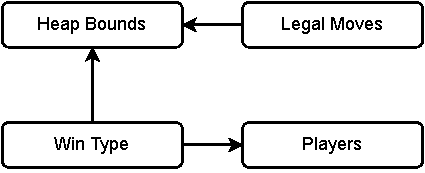
\includegraphics[width=0.6\linewidth]{figures/NimFeatures.pdf}
    \caption{Dependencies between Nim features.}
    \label{fig:nimDependencies}
\end{figure}

We consider a basic two-player (Figure~\ref{fig:nimPlayerFSM}) game using a single, subtractive heap of 5 tokens (Figure~\ref{fig:nimHeapFSM}).
If we view th4 two FSMs operating in lock step for each game move, the game is won when:
\begin{itemize}
    \item the players alternate correctly, as in Figure~\ref{fig:nimPlayerFSM}.  For example, the sequence ABA leads to an accept, but the sequence AAB cannot.
    \item all tokens have been taken, for example using the sequence 212 in Figure~\ref{fig:nimHeapFSM}.
\end{itemize}
Formally, in the theory of regular languages, we seek the \emph{concatenation} of the languages of these two machines.   Given the sequence ABA and 212, each accepted by its respective machine, the concatenation ABA212 is a string in the concatenation of the two languages.  While this correctly represents the sequence of inputs that causes somebody to win, the timing of actions associated with transitions in the two machines does not coincide properly.  For example, it is not possible in the concatenation to determine \emph{who} won the game when the second machine accepts. 

\begin{figure}
    \centering
    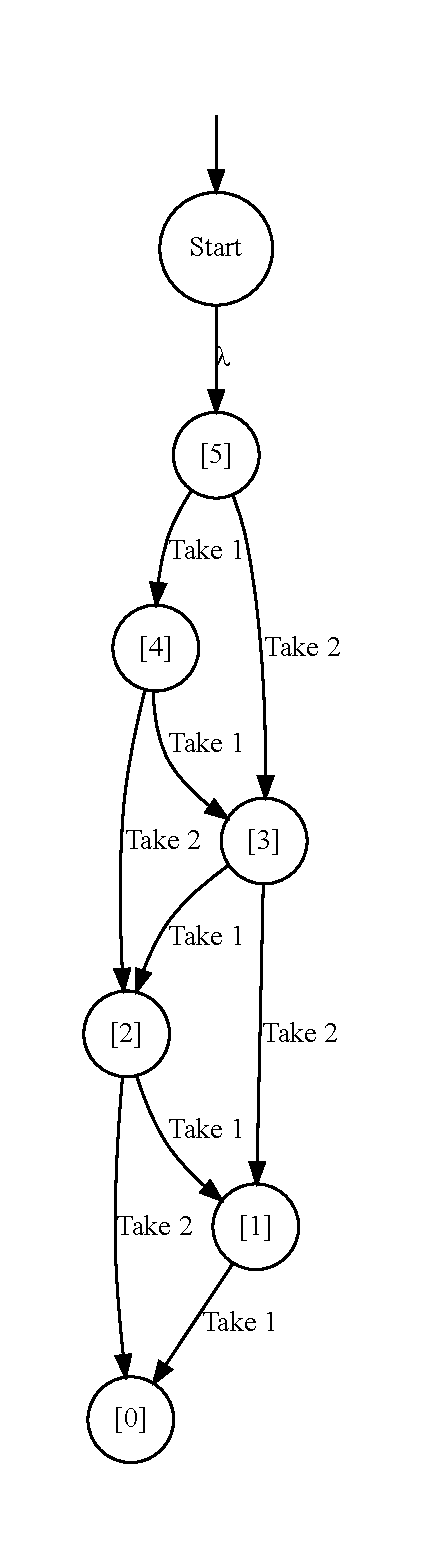
\includegraphics[width=0.55\linewidth]{figures/nimexample/heapFSM.pdf}
    \caption{The Heap finite state machine.}
    \label{fig:nimHeapFSM} 
\end{figure}

We prefer to process the inputs more naturally as (A,2), (B,1), and (A,2), so that the player making the move and the number of subtracted tokens are processed in lock step.  In this way, any actions associated with each move will be properly taken upon that move.  Similarly, if the game had 3~heaps in play instead of a single heap, we want all heaps to be modified by each turn.  Concatenation focuses on one heap until it is exhausted before moving to the next heap.   Finally, consider that the first machine accepts~ABAB which would be inappropriate if the second machine accepts~212, since only~3 moves are made.  The lock-step execution we require is over inputs for each machine that are the same length.

\begin{figure}
    \centering
    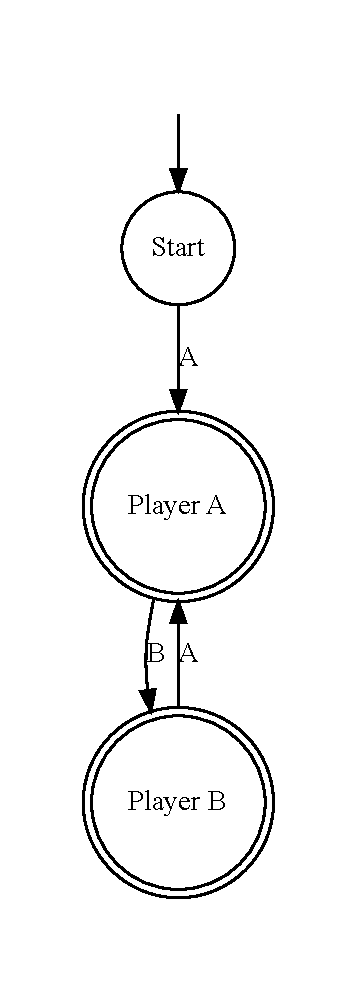
\includegraphics[width=0.35\linewidth]{figures/nimexample/playerFSM.pdf}
    \caption{The Player finite state machine.}
    \label{fig:nimPlayerFSM}
\end{figure}

In support of the semantic actions occurring as they should, and requiring inputs of the same length, we present in Section~\ref{sec:cpalg} an algorithm for constructing a particular \emph{cross product} of two FSMs.  For our example here, the resulting FSM is shown in Figure~\ref{fig:nimFSM}.  This cross product of the Heap and Player machines nicely distinguishes a win by~A from a win by~B, and clearly a move and its player are processed in lock step.

In terms of leverage, consider the cross-product generation of an FSM from two identical FSMS each of size $m$ (states+transitions).  For example, we generate a 2-heap version of Nim by taking the cross product of two such FSMs, as described in Section~\ref{sec:cpalg}.  The resulting machine is of size $O(m^{2})$.  An $n$-way cross product generates a machine of size $O(m^{n})$, where $m$ is viewed as a constant here.  The structures we can generate with this approach are (in the limit) exponential in the size of their specifications.

\begin{figure*}
    \centering
    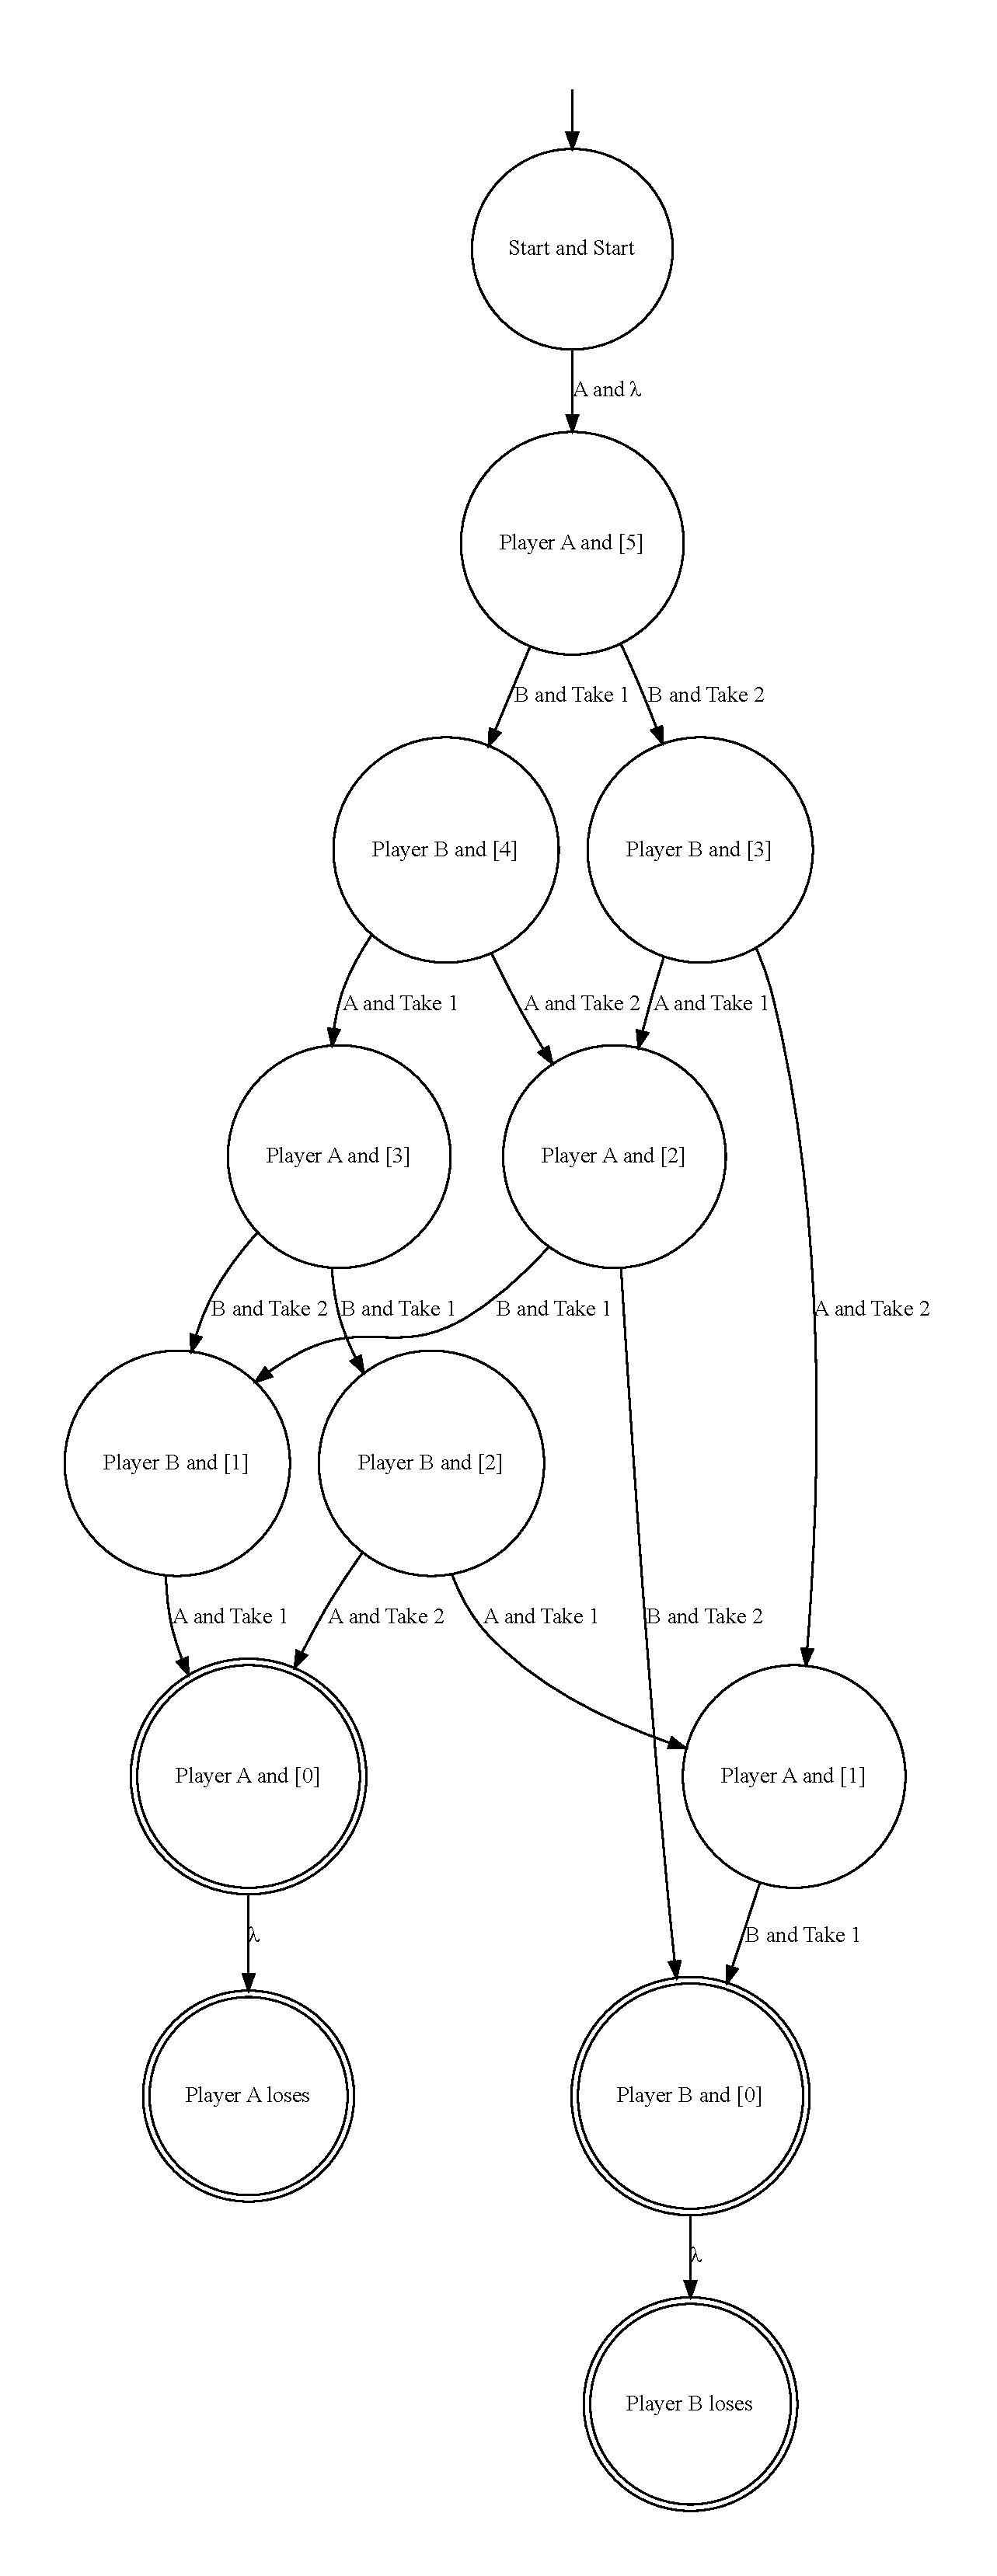
\includegraphics[width=0.45\textwidth]{figures/nimexample/nimFSM.pdf}
    \caption{The resulting Nim finite state machine.  The edge transitions are labeled with the player who acts to take the specified number of tokens. The state is labeled with the player who just completed a turn and the numbefr of remaining tokens.}
    \label{fig:nimFSM}
\end{figure*}

\section{Formalism}\label{sec:formal}
We have developed a formalism to describe both of the feature-decomposition techniques. We begin with an FSM $M$, typically defined as follows: 
\[M = (Q, \Sigma, \delta, q_0, F)\]where $Q$ is a set of states, $\Sigma$ is a set of input symbols, $\delta$ is the transition function, $q_0$ is the start state, and $F$ is the set of accepting states.  A state is typically denoted by an upper-case letter;  lower-case letters denote input symbols and strings.  The symbol $\lambda$ denotes the empty string.  When an FSM is drawn as a graph, the start state receives an edge with no sources, and an accepting state is drawn with two concentric circles. 

The formalisms presented here are implemented in Chisel as a library we call Foam, described in Section~\ref{sec:foam}.  The examples and results presented in this paper were created using Foam.  

\subsection{Cross-cutting features}\label{sec:ccut}
We follow~\cite{aspectsUML} in the treatment of aspects for FSMs.  Essentially a state is like a method and a transition between states is like a method call.  The usual forms of before, after, and around advice are available (\textit{cf}. AspectJ~\cite{AspectJ:01}).   A cross-cutting feature is implemented using advice that modifies an FSMs behavior before, after or during a transition between states.

As described below, a feature is comprised of \emph{advice} applied to \emph{pointcuts} of an FSM, which can formally change the language of the machine, but more broadly the advice can affect actions taken by the machine as its input is processed.  

\paragraph{Pointcuts} These specify \emph{where} advice should be applied in a targeted FSM.   The generative nature of Chisel removes the need for new syntax to express pointcuts.  Instead, we can select states or symbols using simple set quantifiers and predicates, written in Chisel/Scala and executed along with the rest of Chisel code that generates a circuit.  For example, the \textbf{Print Funds} feature can be generated in a vending-machine FSM through \emph{after} advice applied to any token that adds value to the machine.  Such properties are implemented nicely in Scala using \emph{traits}.  To implement this feature, the base code likely requires refactoring to include the value trait.  However, the effort is worthwhile because the refactoring and associated advice make the resulting product both clearer and more easily able to exclude or include actions taken at different inputs.

In AOP terminology, a pointcut yields a set of \emph{joinpoints} at which advice is applied.  A joinpoint associated with the above example would be a single token~``5'', such at the one between state ``10'' and ``15'', at which the value increase in the machine by ``5'' cents.  Because this is an \emph{after} pointcut, the joinpoint has context that includes the state~``15'' that follows the token~``5'', as shown in Figure~\ref{fig:vend1}. 

\begin{figure*}
    \centering
    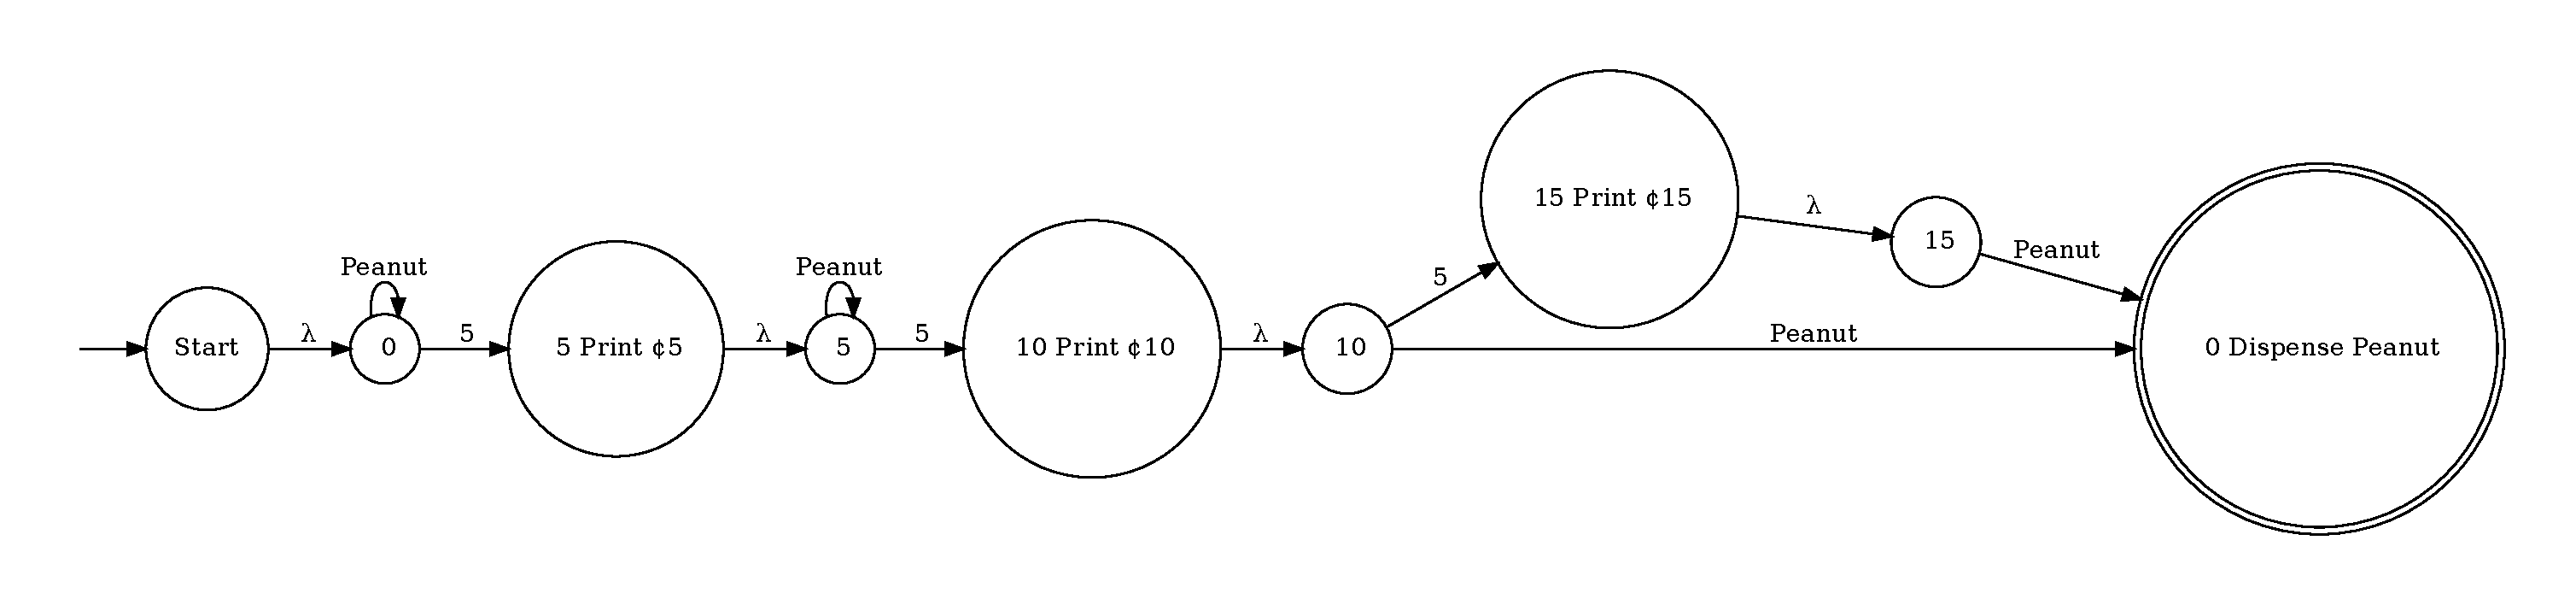
\includegraphics[width=0.8\textwidth]{figures/vend2.pdf}
    \caption{The resulting FSM of the application of Print Funds to the FSM from Figure \ref{fig:vend1}.}
    \label{fig:applyadvice}
\end{figure*}

\paragraph{Advice} This specifies \emph{what} changes to the FSM should be applied at a joinpoint. In the \textbf{Print Funds} feature, a new state is inserted following each token~``5'' in the FSM. The exact print statement generated by the advice is determined by the context contained within the joinpoint. For example, \texttt{Print \textcent15} because the state~``15'' follows the token~``5'' discussed earlier. Furthermore, to prevent infinite application of features, the advice for \textbf{Print Funds} checks to see if the context in the joinpoint is already a printing state. If so, no advice is applied.

Like pointcuts, advice is written in Chisel/Scala. Not only can advice insert new states, but it can also insert new symbols as well. Take the \textbf{Print Funds} feature for example. The pointcut is predicated upon a dispense state having a ``peanut'' trait. Because this is a \emph{before} pointcut, each joinpoint has context that includes each path into the state. In Figure \ref{fig:applyadvice2} this is $10 \xrightarrow{Peanut}$ and $15 \xrightarrow{Peanut}$. The advice will insert a new ``Contains Nuts!''~state and ``Accept''~token for each of the joinpoints. It also inserts a new transition on the ``Reject''~token whose destiation is determined by the context contained in the joinpoint.

\begin{figure*}
    \centering
    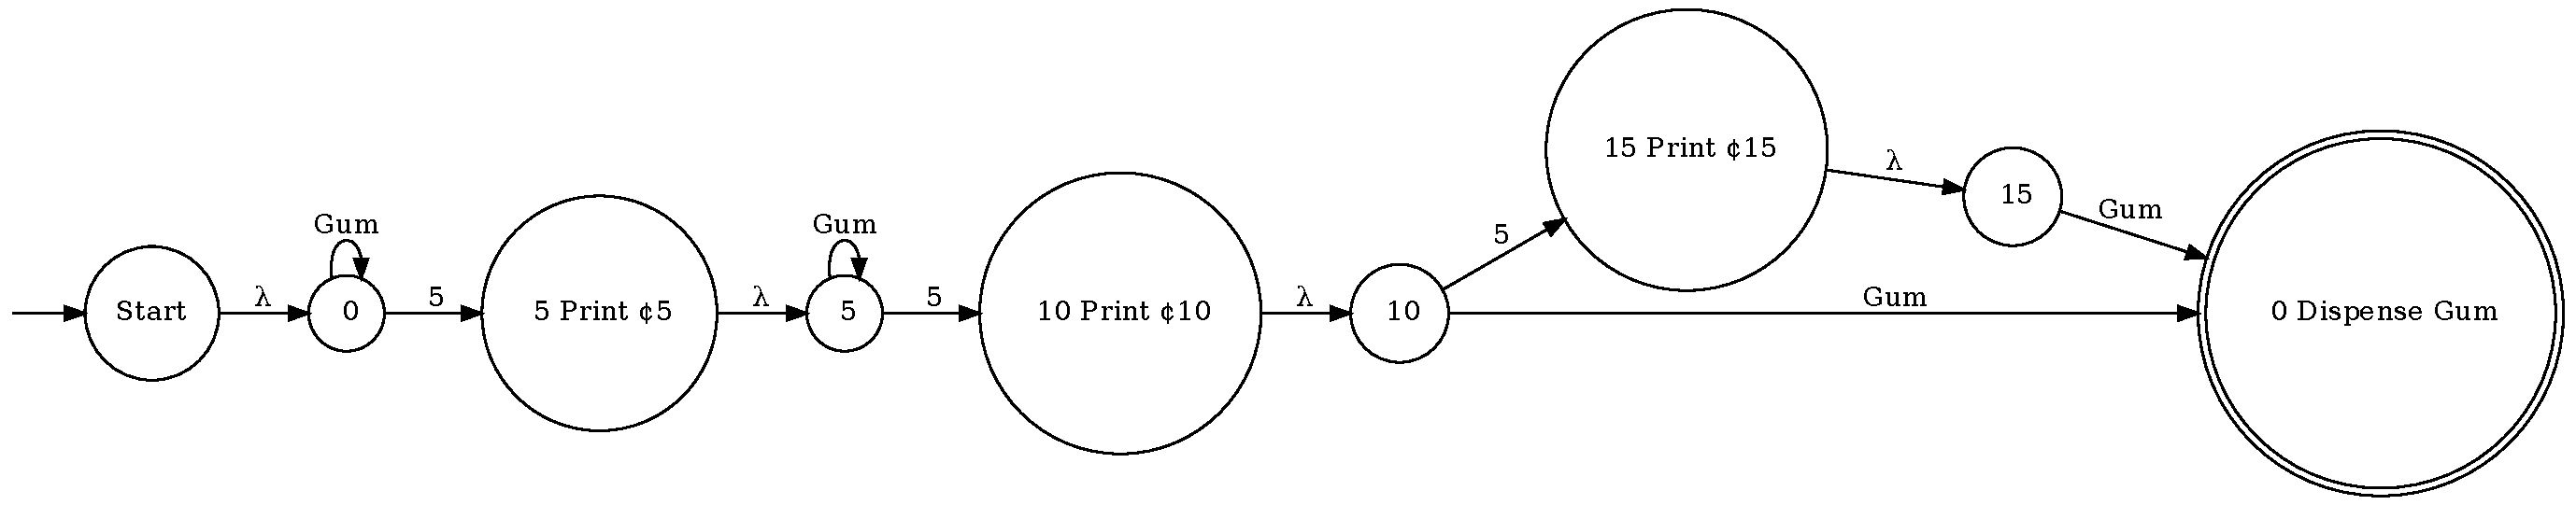
\includegraphics[width=0.8\textwidth]{figures/vend3.pdf}
    \caption{The resulting FSM of the application of Peanut Warning to the FSM from Figure \ref{fig:vend1}.}
    \label{fig:applyadvice2}
\end{figure*}

\subsection{Cross-product features}\label{sec:cpalg}
\pnote{Should this be Cross-product Features? OR should this be on the cross product machines?}

Below we present the algorithm for producing the lock-step, cross-product finite state machine from two deterministic finite state automata. 

\begin{figure}[htb]
\renewcommand{\algorithmicrequire}{\textbf{Inputs:}}
\renewcommand{\algorithmicensure}{\textbf{Output:}}
\renewcommand\thealgorithm{}
\begin{algorithmic}[1]
\REQUIRE {$A = (Q_A, \Sigma_A, \delta_A, q_A, F_A), B = (Q_B, \Sigma_B, \delta_B, q_B, F_B)$}
\ENSURE {$C = (Q_C, \Sigma_C, \delta_C, q_C, F_C)$}

\STATE{$q_C \gets (q_A, q_B)$}
\STATE{$Q_C \gets \{q_C\}$}
\STATE{$L \gets \{q_C\}$} \hfill\COMMENT{Work queue}
\STATE{$P \gets \emptyset$} \hfill\COMMENT{Already-processed states}
\WHILE{$L \neq \emptyset$}
    \STATE{$s = (s_A, s_B) \gets \mathrm{dequeue}(L)$}
    \STATE{$P \gets P \cup \{s\}$}
    \FOR{$(s_A \xrightarrow{a} d_A \in \delta_A) \times (s_B \xrightarrow{b} d_B \in \delta_B)$}
        \STATE{$d \gets (d_A, d_B)$}
        \IF{$d \not\in P$}
            \STATE{$L \gets L \cup \{d\}$}
        \ENDIF
        \STATE{$\delta_C(s, (a, b)) \gets d$} 
        \IF{$d_A \in F_A \land d_B \in F_B$}
            \STATE{$F_C \gets F_C \cup \{d\}$}
        \ENDIF
    \ENDFOR
\ENDWHILE
\end{algorithmic}
\caption{Construction of the Cross Product FSM.  The inputs $A$ and $B$ must be deterministic;  the output $C$ is deterministic.}\label{fig:algo}
\end{figure}

This algorithm works as a breadth-first search of both machines, maintaining a work queue of combined-states that still need to be processed. Starting with the combined-state of the individual machines' starting states, the cartesian product of transitions is considered. Combined destination states are added to the work queue if they have not yet been processed. The algorithm then iteratively constructs the transition function by adding the transition $s \xrightarrow{(a,b)} d$, and constructs the concomitant set of states and alphabet. Each combined destination state is marked as an accepting state if both of the component destination states are accepting states. 

Consider this algorithm applied to Figures~\ref{fig:nimPlayerFSM} and \ref{fig:nimHeapFSM}, with $L = \{(\text{Player A}, [5])\}$. In this case, $s = (\text {Player A}, [5])$; it is added to the already-processed states list $P$, and then we consider the Cartesian product of transitions from state $\text{Player A}$ in the player machine and from state $[5]$ in the heap machine. This gives us $\{\text{Player A} \xrightarrow{B} \text{Player B}\} \times \{[5] \xrightarrow{\text{Take } 1} [4], [5] \xrightarrow{\text{Take } 2} [3]\}$. First consider the pair of transitions $(\text{Player A} \xrightarrow{B} \text{Player B}, [5] \xrightarrow{\text{Take } 1} [4])$: the combined destination state is $(\text{Player B}, [4])$. As the combined destination state is not already in $P$, it is added to the work queue $L$. The transition $(\text {Player A}, [5]) \xrightarrow{(B, \text{Take } 1)} (\text{Player B}, [4])$ is added to the cross product machine's transition function, with the state $(\text{Player B}, [4])$ being added to $Q_C$ and $(B, \text{Take } 1)$ being added $\Sigma_C$. As $[4]$ is not an accepting state, their destination state is not added to $F_C$. Then, $(\text{Player A} \xrightarrow{B} \text{Player B}, [5] \xrightarrow{\text{Take } 2} [3])$ would be processed similarly. \pnote{Is it worth adding $X$ state would be added to $L$, $Y$ to $P$, etc?}

% The algorithm begins by combining the two starting states and adding it to the work queue. It then proceeds by removing the first entry from the work queue, splitting it into its two component states, and iterates through all combinations of transitions from the component states within their respective machines. For each pair of transitions, their destination states are combined into a composite state, and is marked for later processing. Then, the cross product machine's transition function is augmented to include this transition, and the resulting state is marked as an accepting state if both component states are likewise accepting. 




\section{Aspect Oriented Finite State Machine Library}\label{sec:foam}
We have implemented an aspect oriented finite state machine library, which we call Foam,  in Scala\footnote{https://github.com/wustl-frisc/foam}. In this section, we detail the library as well as code generation.

While Foam is not a fully fledged domain specific language, we have modeled the interface after the well established aspect-oriented extension to Java, AspectJ~\cite{}. The intention is to give aspect-oriented practitioners a familiar interface for interacting with the finite state machines. Since the library is implemented in plain Scala, we have access to and utilize the full powers of the type system. Following our vending machine example, Figure~\ref{lst:PrintFunds} shows the implementation of the \textbf{Print Funds} feature in Foam.

We provide a series of extendable base classes to represent finite state machines. The library takes care of building pointcuts, applying aspects, and performing the cross-product. We have even provided reflexive access, just like AspectJ to the join-point and its incoming and outgoing paths. Given this, in relatively few lines of code, programmers can create advice with ease.

\begin{figure*}
    \centering
    \begin{lstlisting}[language = Scala]
class PrintFunds extends Aspect[NFA] {
  def apply(nfa: NFA) = {

    val tokenPointcut = Pointcutter[Token, Coin](nfa.alphabet, token => token match {
      case t: Coin => true
      case _ => false
    })

    AfterToken[Coin](tokenPointcut, nfa)((thisJoinpoint: TokenJoinpoint[Coin], thisNFA: NFA) => {
      var value = thisJoinpoint.out.asInstanceOf[ValueState].value
      thisJoinpoint.out match {
        case s: PrinterState if (s.action == "Funds:" + value.toString) => (None, thisNFA)
        case _ => (Some((PrinterState("Funds:" + value, value, false), Lambda)), thisNFA)
      }
    })
  }
}
\end{lstlisting}
    \caption{The implementation of the Print Funds feature in Foam.}
    \label{lst:PrintFunds}
\end{figure*}

\subsection{Code Generation}
The library currently supports emitting GraphVis and Verilog code. Code generation is decoupled from the creation of the finite state machines, as the library generates code based off the internal data structures, not the Scala code itself. Code GraphVis and Verilog code are generated by Graphviz4S~\cite{} and Chisel, respectively. 

\section{Case studies and results}\label{sec:results}
Here we present three case studies to demonstrate the generative ability of our framework: a Vending Machine, the game of Nim, and SIMD cache coherence.

\subsection{Vending Machine}\label{sec:vendresults}
We implemented all the features from Section \ref{sec:vend} in our library. The resulting FSMs were then emitted as Verilog. The Verilog was then synthesized on a xc7a35tcpg236-1 FPGA using Vivado 2022.1. Below we report the number of generated states, transitions in the FSM, and the space in LUTs that the FSM took up in on the FPGA.

Figure \ref{fig:vmData} shows the results for different endpoints generated by our library. For our tests, we held the currency threshold at 100. Every machine contains 5, 10, 25 value coins and 4 products of value 25, 50, 75, and 100. This is captured by \textit{None}. In the first set of results, each feature is shown by itself. Even single features can greatly increase the components in the FSM. The \textbf{Buy More} feature (denoted B) by itself more than doubles the number of states and transitions. This impressive leverage is further exemplified when combining features. 

In these cases the number of states increase by 2.5x in the simplest endpoint up to 4.6x in the most complex, and the transitions by 2.5x and 5x respectively. Recall, this is in a relatively simple vending machine that can only accept up to 100 units of value. Simply doubling the amount of accepted value to 200 creates a machine with 284 states (10.5x increase over the base) and 3113 transitions (16x increase over the base). However, this is accomplished in our library with relatively few lines of code. The largest feature in terms of code is \textbf{Peanut Warning}, which is implemented in just 39 lines. \jnote{Report the lines of code for each feature?}

Despite the huge number of generated states and transitions, the resulting LUTs taken up by the FSM are linear. This is due to the fact that hardware synthesis tools can encode the states using a linear scheme. However, the original specification of that circuit \textit{must be expressed in the exponential form first} for the synthesis tools to recognize it. With our framework, hardware designers are not limited to small finite state machines.

\begin{figure}
    \centering
\begin{tabular}{lrrrr}\toprule
Features &States &Transitions &LUTs \\\midrule
None &27 &208 &24 \\
P &47 &368 &38 \\
I &47 &368 &46 \\
C &48 &423 &70 \\
W &33 &320 &60 \\
B &57 &448 &60 \\
PI &67 &528 &73 \\
PICB &118 &1053 &186 \\
PICW &94 &1023 &160 \\
PICWB &124 &1353 &220 \\
\bottomrule
\end{tabular}
    \caption{Number of generated states, transitions, and LUTs depending on selected features. The features are as follows: P = Print Funds, I = Insufficient Funds, C = Change Return, W = Peanut Warning, and B = Buy More.}
    \label{fig:vmData}
\end{figure}

\subsection{Nim}\label{sec:nimresults}
\todo{Removed ``tokens'' from the data.}
\paragraph{Traditional Nim}
The classical game of Nim is a mis\`{e}re game of two players and a finite number of heaps. Each turn, the current player may only remove tokens from a single heap of their choosing, and must take between 1 and all the tokens remaining in that heap. 

In the simplest variation of traditional Nim, with a single heap containing three tokens and only allowing one player, six states and five tokens were created, as seen in Figure~\ref{tab:traditionalNim}. However, the results quickly explode as the number of players increase, and predominately, as the number of heaps and their initial quantities of tokens increases. Allowing for three heaps, containing 3, 4, and 5 tokens respectively, and having two players -- a common example used to introduce Nim -- already contains 235 states, 26 tokens, and 6110 transitions. 

\begin{figure}
\small
\begin{tabular}{rrrrrrrr}\toprule
\multicolumn{3}{c}{Heaps} &Players &States &Tokens &Transitions \\\cmidrule{1-7}
3 &4 &5 & & & & \\\midrule
\checkmark & & &1 &6 &5 &30 \\
\checkmark & & &2 &9 &7 &63 \\
\checkmark & & &4 &11 &8 &88 \\
\checkmark &\checkmark & &1 &22 &9 &198 \\
\checkmark &\checkmark & &2 &39 &16 &624 \\
\checkmark &\checkmark & &4 &60 &30 &1800 \\
\checkmark & \checkmark &\checkmark &1 &112 &14 &1708 \\
\checkmark & \checkmark &\checkmark &2 &235 &26 &6110 \\
\checkmark & \checkmark &\checkmark &4 &419 &50 &20950 \\
\bottomrule
\end{tabular}
\caption{Number of generated states, tokens, and transitions by selected features for traditional Nim. Each game was played as Mis\`{e}re play.}\label{tab:traditionalNim}
\end{figure}

\paragraph{The Subtraction Game}
The Subtraction game is a single heap variation of Nim, usually played by a small group of players. The players take turns in a round-robin style and remove between one and a pre-determined number of tokens. As the game is played as a Mis\`{e}re game, the player taking the final token loses. 

\begin{figure}
\small
\begin{tabular}{cccrrrrr}\toprule
\multicolumn{3}{c}{Allowed} & & & & \\
\multicolumn{3}{c}{Moves} &Players &States &Tokens &Transitions \\\cmidrule{1-7}
-1 &-2 &-3 & & & & \\\midrule
\checkmark & & &1 &24 &3 &72 \\
\checkmark & & &2 &24 &4 &96 \\
\checkmark & & &4 &24 &6 &144 \\
\checkmark &\checkmark & &1 &24 &4 &96 \\
\checkmark &\checkmark & &2 &45 &6 &270 \\
\checkmark &\checkmark & &4 &81 &10 &810 \\
\checkmark & \checkmark &\checkmark &1 &24 &5 &120 \\
\checkmark & \checkmark &\checkmark &2 &45 &8 &360 \\
\checkmark & \checkmark &\checkmark &4 &83 &14 &1162 \\
\bottomrule
\end{tabular}
\caption{Number of generated states, tokens, and transitions for the Subtraction game. Every game is played with a single starting heap of 21 tokens and through Mis\`{e}re play. }\label{tab:subtractionNim}
\end{figure}

\paragraph{Circle Nim}
Circle Nim is a variation of Nim where the heaps are placed around a circle. Each turn, players are allowed to take tokens from between one and an upper-bounded quantity of consecutive heaps, taking between one and every token within each heap. This is often played as a mis\`{e}re game. 

\begin{figure}
\small
\begin{tabular}{cccrrr}\toprule
Heaps &Players &States &Tokens &Transitions \\\midrule
3 &1 &10 &11 &110 \\
3 &2 &15 &17 &255 \\
3 &4 &17 &20 &340 \\
6 &1 &66 &20 &1320 \\
6 &2 &113 &38 &4294 \\
6 &4 &150 &74 &11100 \\
9 &1 &514 &29 &14906 \\
9 &2 &951 &56 &53256 \\
9 &4 &1429 &110 &157190 \\
\bottomrule
\end{tabular}
\caption{Number of generated states, tokens, and transitions by variation of features for Circle Nim. Each heap contained one token, players could take between one and three consecutive tokens, and all games were played as Mis\`{e}re play. }\label{tab:circleNim}
\end{figure}

\subsection{SIMD Caches}\label{sec:cache}
Ultimately, the goal of this work is to make the design of complex hardware easier through generation. Here, we will demonstrate how we can combine our techniques with ``off the shelf'' components to generate SIMD Caches that are coherent with each other. While we recognize that this is purely a pedagogical example, it is modeled off the real-world RDNA Architecture from AMD~\cite{}.

The RDNA architecture packages two SIMD execution units into a single unit called a \textit{work-group processors}. Each work-group shares L0 cache between each SIMD unit. This cache is kept coherent through serialization of the execution when conflicts are detected. Two work-groups are then packaged together into a \textit{Dual Compute Unit} (DCU). Currently, the two L0s within a DCU are kept coherent via software. 

Suppose that we wanted to model a similar cache system ourselves, but instead of handling data conflicts between the two SIMD units in a work-group processor, we use the MSI cache coherence protocol~\cite{}. For this case study, we have selected the ready-made cache from RISC-V Mini~\cite{}. As-is, this cache, shown in Figure \ref{fig:cacheBefore}, is directly connected to main memory in a single core system and does not have any coherence protocol. Using a feature oriented approach, we can retrofit this cache with advice that implements the MSI protocol, shown in Figure \ref{fig:cacheAfter}. In order to model the interactions between the two now coherent caches, we can cross-product the two. This results in an FSM with 729 states, 3,376 tokens, and 2,461,104 transitions. Hardware designers could use this sort of modeling for correctness verification, however that is beyond the scope of this paper.

\begin{figure}
    \centering
    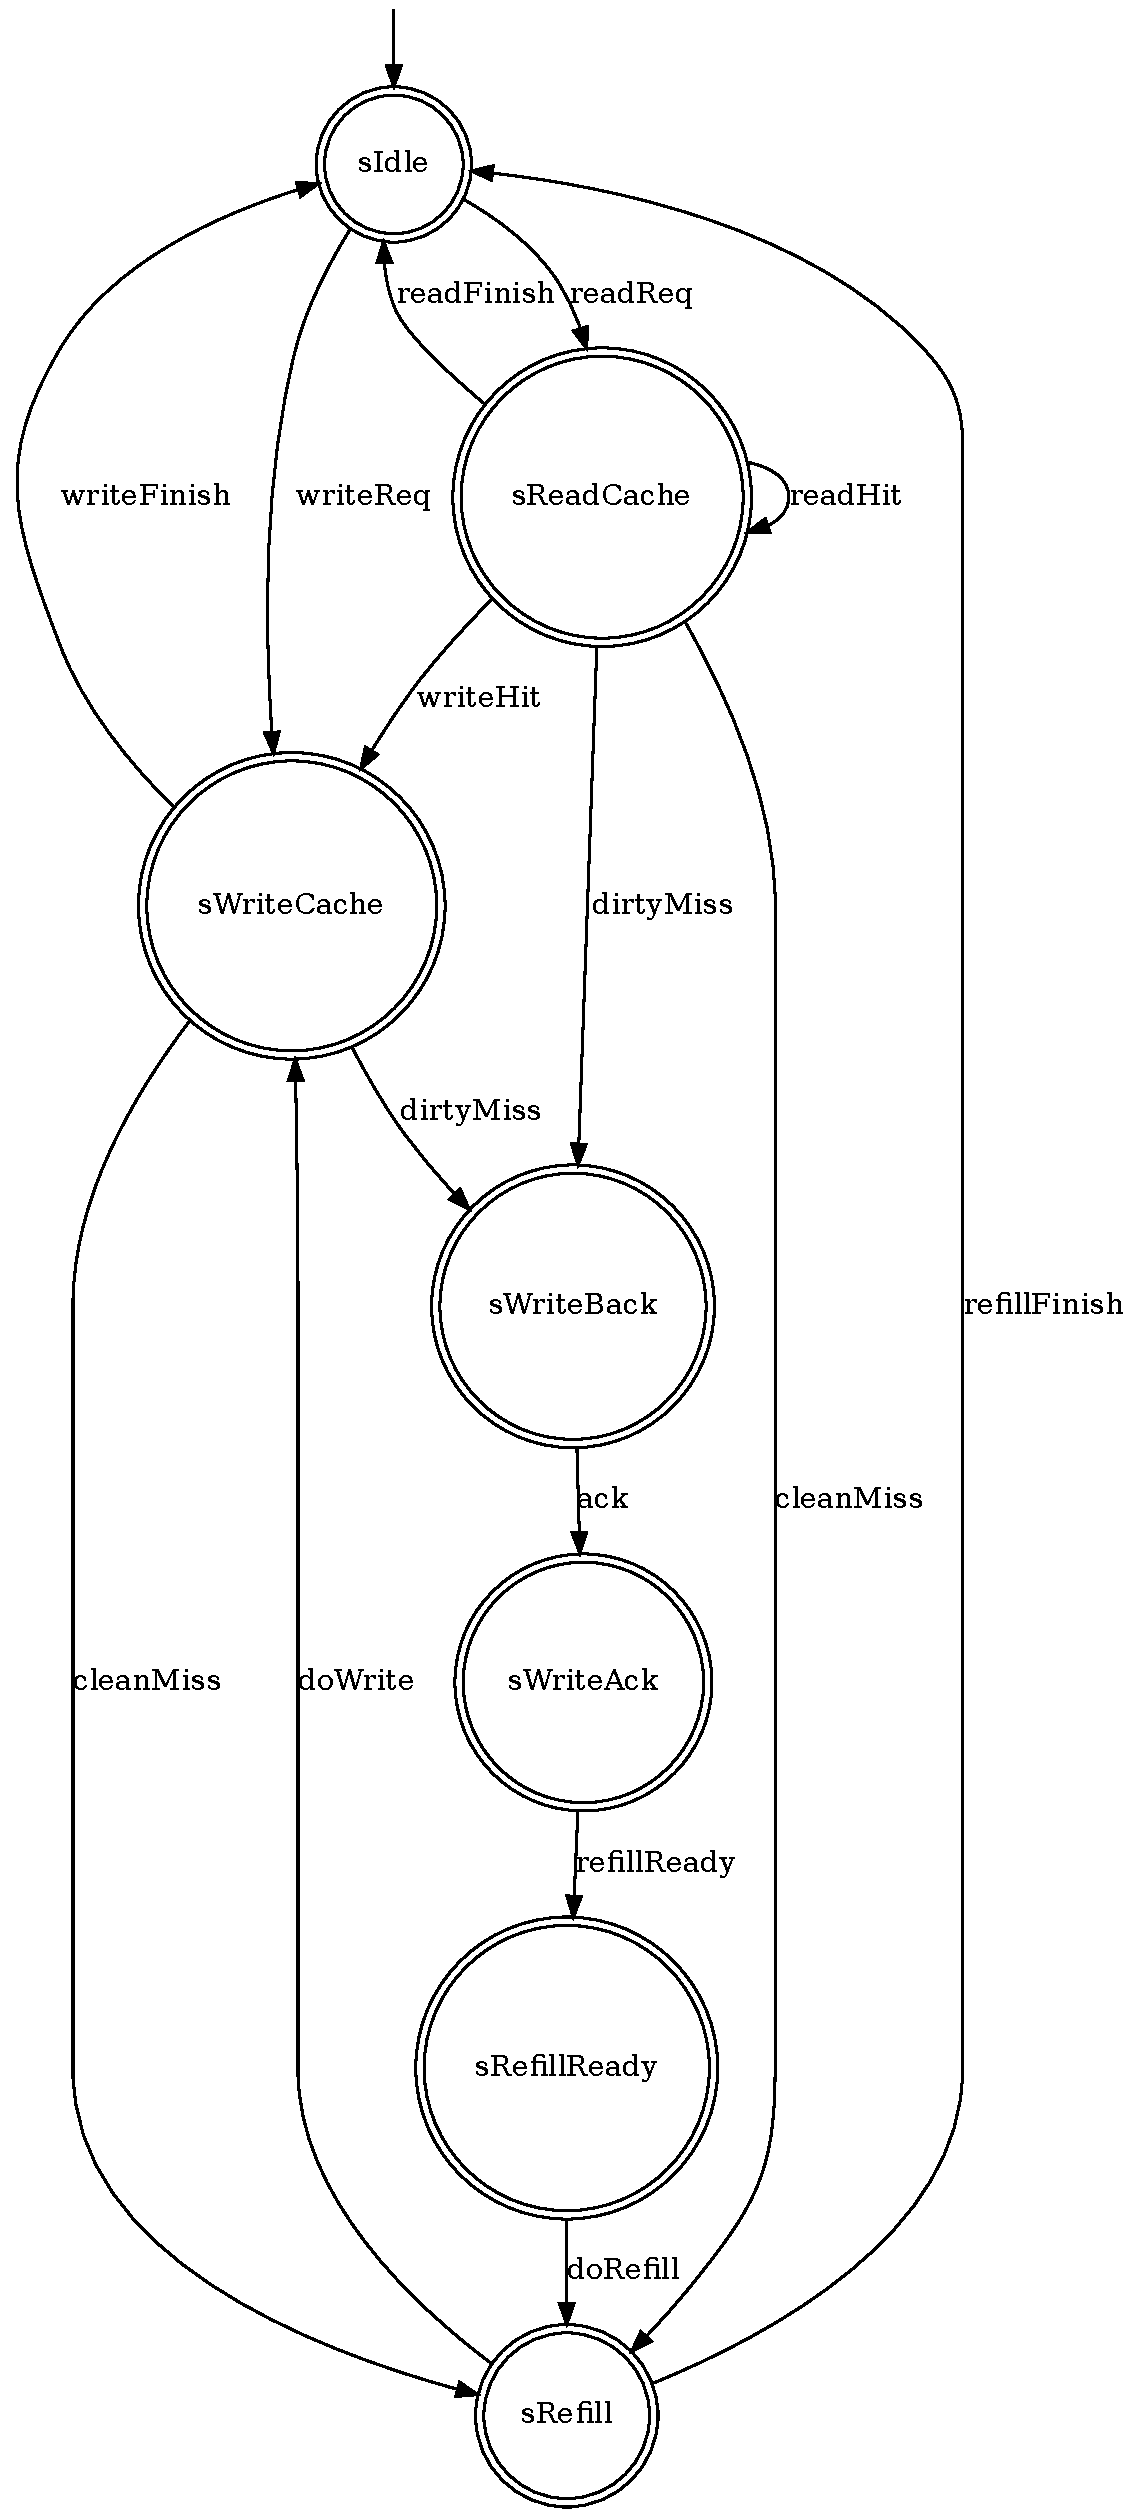
\includegraphics[width=0.7\linewidth]{figures/cacheFSM.pdf}
    \caption{The cache FSM from the RISC-V Mini.}
    \label{fig:cacheBefore}
\end{figure}

\begin{figure*}
    \centering
    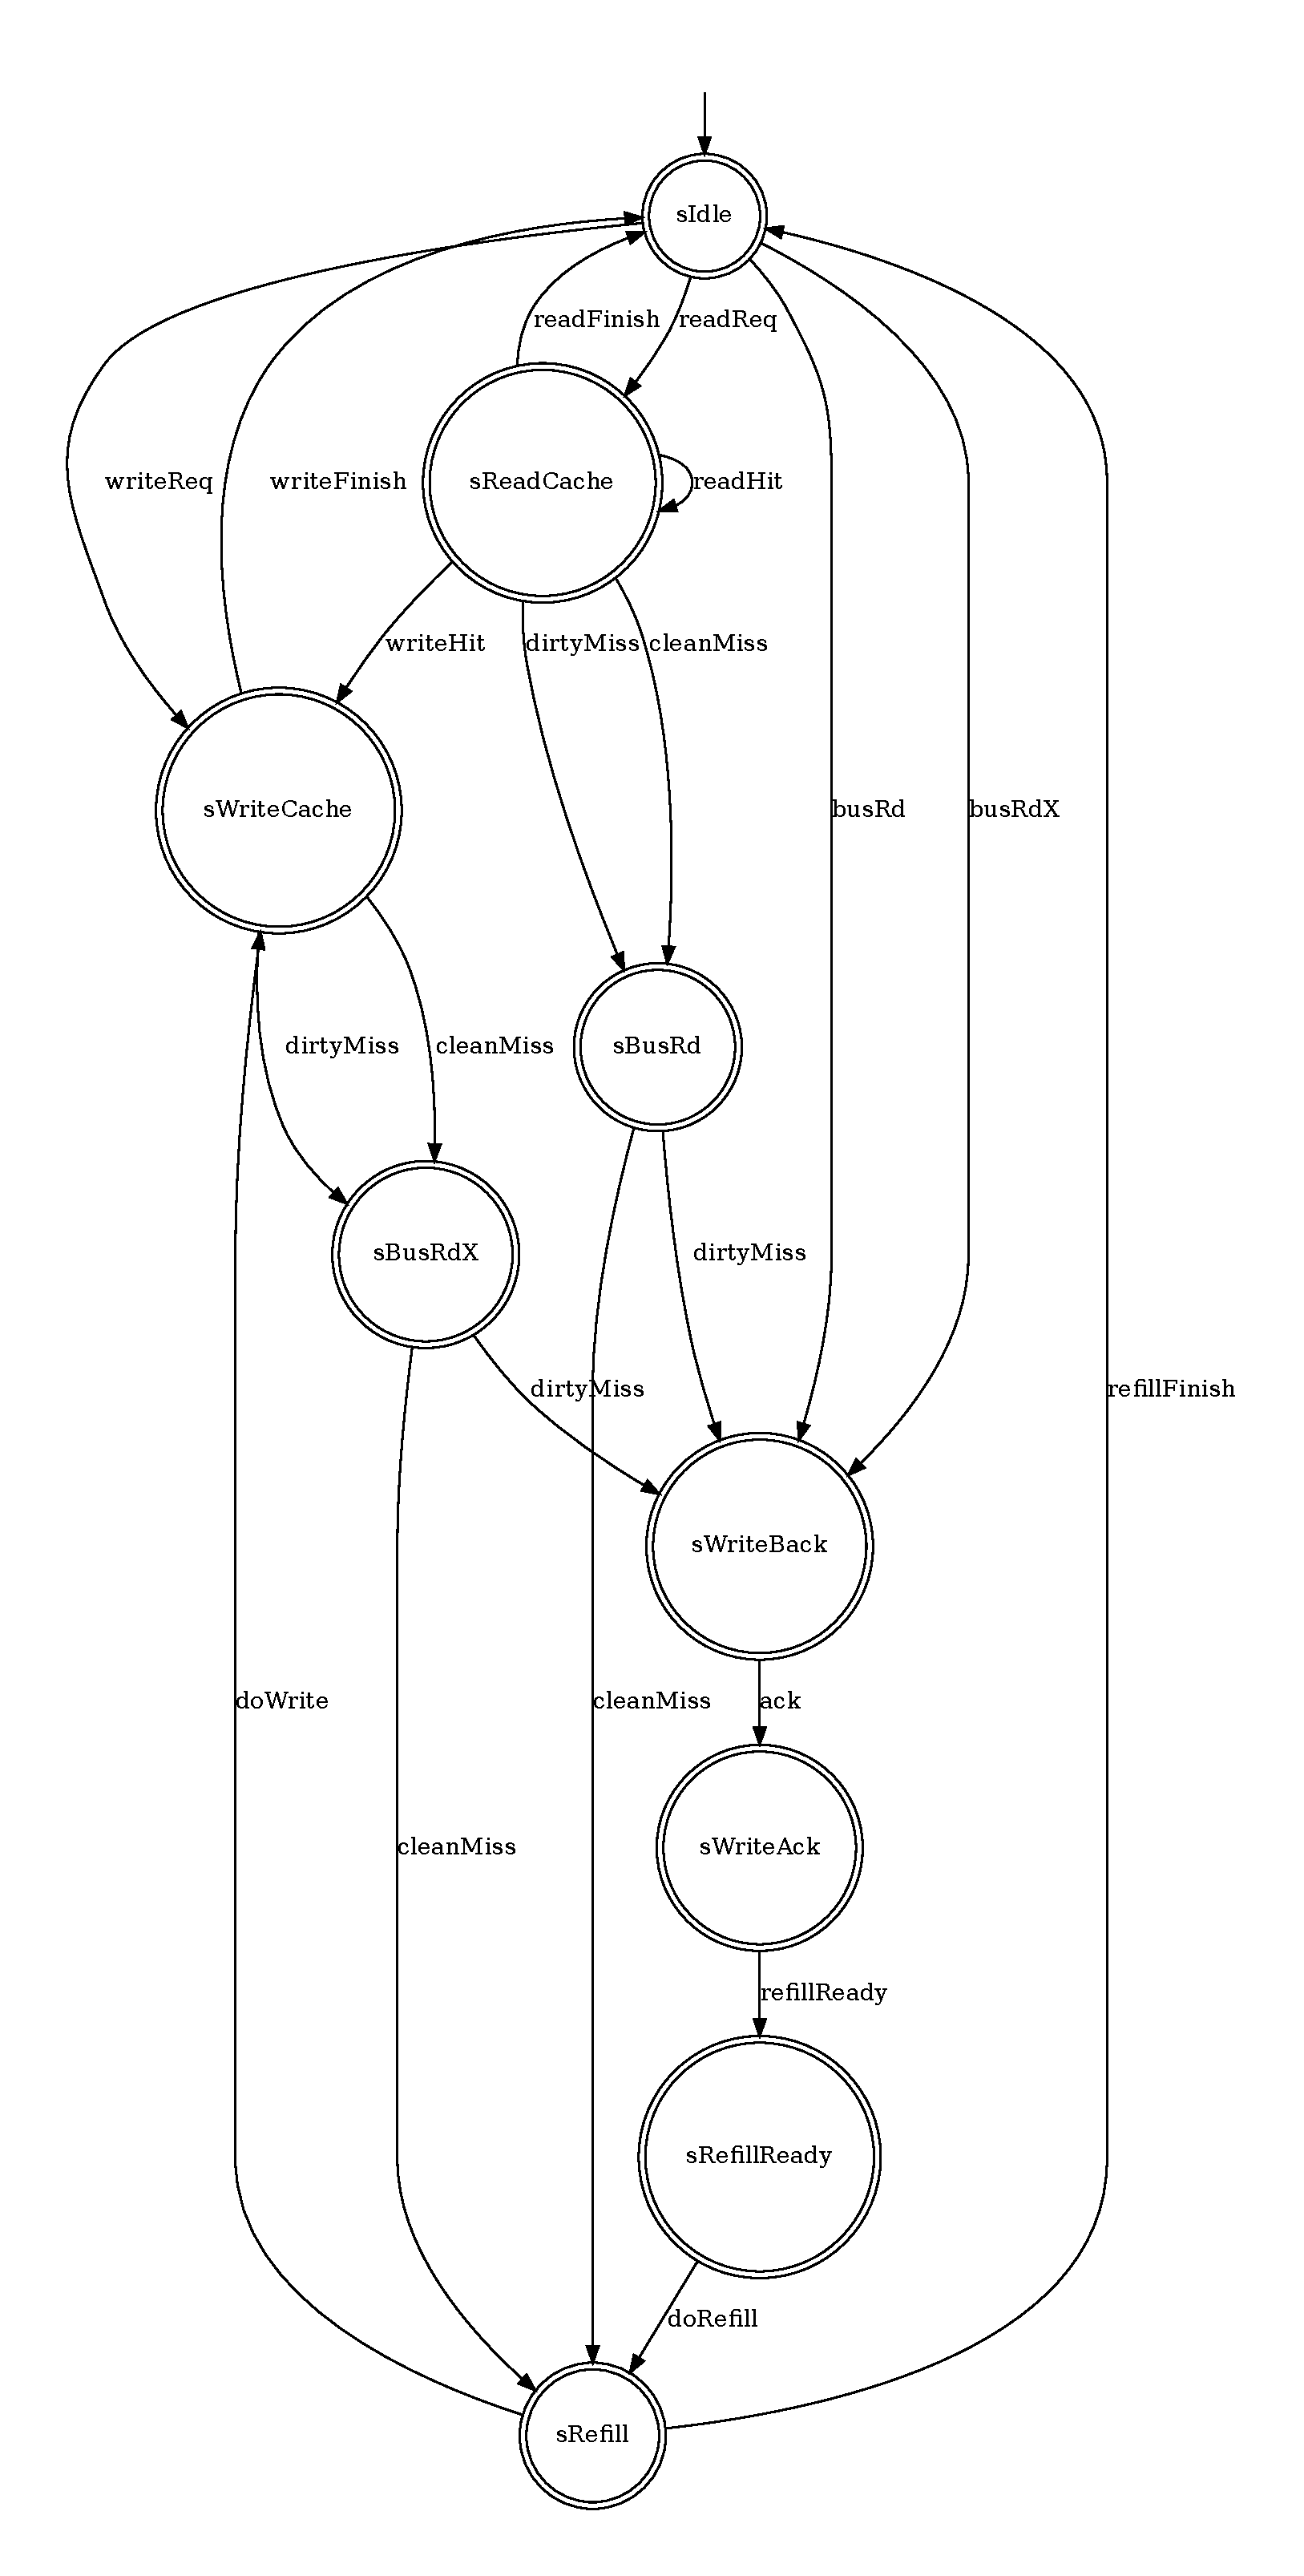
\includegraphics[width=0.5\linewidth]{figures/cacheFSM2.pdf}
    \caption{The cache FSM from RISC-V Mini with the MSI protocol.}
    \label{fig:cacheAfter}
\end{figure*}

Imagine that in the next iteration of the architecture, the designers wanted to use hardware coherence between all the SIMD units in a DCU rather. Instead of having to start the model completely from scratch, hardware designers can simply instantiate two more caches into the system. Furthermore, instead of being locked into a single cache coherence protocol, the hardware designers may want to choose the MESI protocol~\cite{}, for their next iteration. With our approach, this protocol can just be applied instead of the MSI protocol. 

\section{Future Work}
In future work, we plan on creating a fully feature-oriented cache using our system. Hardware caches are ripe for feature-oriented design as they contain many orthogonal features. For example, if we wanted to build a cache model even closer to the RDNA architecture, the original cache FSM would need to be write-through, 4-way set associative, and utilize an LRU replacement policy. Instead of forcing hardware designers into choosing an initial design and refactoring, write policy, allocation policy, replacement policy, and associativity could all be selectable features of the microarchitecture.

Beyond just the cache, it is easy to extend this concept of feature-oriented hardware design to the chip as a whole. Hennessy and Patterson's original motivation behind the RISC-V architecture was to create an open and \textit{modular} instruction set. RISC-V is used in small application specific processors such as the controllers for Western Digital storage products~\cite{} and Google's Titan M2 security chip~\cite{}; all the way up to high performance application processors such at the SiFive P650~\cite{}. Instead of independently implementing each of these endpoints of RISC-V and the microarchitecture, we posit that featureful implementation of RISC-V would be far more useful. In this world, hardware designers could swap in and customize each of the ISA and microarchitectural features they need. This could open up a marketplace for hardware feature exchange. This is something that the software community has enjoyed for over a half century.

%%
%% The next two lines define the bibliography style to be used, and
%% the bibliography file.
\bibliographystyle{ACM-Reference-Format}
\bibliography{acmart,bibdbase,networks}

\end{document}
\endinput
%%
%% End of file `sample-sigplan.tex'.
